\documentclass{article}

\usepackage[final]{neurips_2026}

\usepackage[utf8]{inputenc}
\usepackage[T1]{fontenc}
\usepackage{hyperref}
\usepackage{url}
\usepackage{booktabs}
\usepackage{amsfonts}
\usepackage{amsmath}
\usepackage{graphicx}
\usepackage{microtype}
\usepackage{xcolor}

\title{Predicting Professional Tennis Match Outcomes with Pre-Match Data}

\author{%
  Yining Chen\\
  CS 439: Introduction to Data Science\\
  Section 7; NetID: \texttt{ycc30}
  \And
  Michael Chiu\\
  CS 439: Introduction to Data Science\\
  Section 7; NetID: \texttt{mkc149}
  \And
  Ryan Xu\\
  CS 439: Introduction to Data Science\\
  Section 7; NetID: \texttt{rwx1}
}

\begin{document}

\maketitle

\begin{abstract}
Professional tennis is a useful prediction setting because each match has a clear binary outcome, rich public historical data, and many interpretable pre-match covariates. We study ATP singles matches from 2010 through 2024 and ask whether ranking, ranking points, age, surface, round, match format, experience, and prior win-rate features can predict winners more accurately than a simple higher-ranked-player baseline. The raw Jeff Sackmann ATP match files contain 42,571 matches; after basic date and ranking cleaning, our modeling dataset contains 41,750 matches. To avoid target leakage, we rewrite each match as a randomized Player 1 versus Player 2 prediction problem and construct all history features using only matches that occurred earlier in time. We compare logistic regression, random forest, and gradient boosting pipelines using five-fold time-series cross-validation. The higher-ranked baseline achieves 65.3\% mean accuracy and 0.690 ROC-AUC. The random forest performs best among the learned models, reaching 66.6\% mean accuracy, 66.6\% balanced accuracy, 66.9\% F1, and 0.732 ROC-AUC. Feature importance suggests that ranking points, ranking difference, career win rate, and surface-specific win rate are the most informative inputs. These results show that simple pre-match features improve slightly over rankings alone, but also that tennis outcomes remain noisy and difficult to predict without richer player, injury, scheduling, and match-context information.
\end{abstract}

\section{Introduction}

Predicting the winner of a professional tennis match is both intuitive and challenging. The outcome is a clean binary label, and the sport provides detailed historical records for each event, surface, player ranking, and match result. At the same time, tennis is full of short-term variation: a player can have a poor serving day, carry fatigue from a long previous round, return from injury, or match up unusually well against a higher-ranked opponent. This makes tennis a good case study for introductory data science because the task is simple to state but still requires careful data cleaning, feature construction, leakage prevention, modeling, and evaluation.

Our project asks: \emph{which pre-match factors most strongly influence the outcome of a professional tennis match, and how accurately can we predict the winner using rankings, recent form, court surface, and historical performance?} We began with the common expectation that rankings should be highly predictive. ATP rankings summarize recent tournament performance and therefore act as a public estimate of player strength. However, rankings are not designed as match-specific forecasts. They do not directly encode whether a player is especially strong on clay, whether a player has accumulated wins recently, whether the players are close in ranking points despite different rank numbers, or whether the match is a best-of-five Grand Slam contest rather than a best-of-three tour match.

The project therefore has two goals. The first is predictive: compare several standard machine-learning models against a ranking-only rule. The second is interpretive: identify which engineered features the strongest model uses most. Because this is a final course project rather than a production betting system, interpretability and methodological honesty are more important than squeezing out every possible percentage point of accuracy. We intentionally exclude same-match statistics such as aces, double faults, break points saved, and serve points won because those values are only known after the match and would leak the answer into the predictors.

Our central finding is that learned models can improve on a ranking-only baseline, but the improvement is modest. Across five time-ordered validation folds, the higher-ranked-player rule achieves 65.3\% accuracy. A random forest trained on ranking, points, age, experience, surface, round, format, and prior win-rate differences reaches 66.6\% accuracy and a stronger ROC-AUC of 0.732. The gap is not enormous, but it is meaningful because every feature used by the learned models is available before match start. The feature-importance analysis also gives a coherent story: ranking points and ranking gap remain central, while career and surface-specific win rates add information beyond rank.

The rest of the paper is organized as a standard empirical research report. Section~\ref{sec:related} summarizes related work and modeling ideas. Section~\ref{sec:data} describes the data and preprocessing. Section~\ref{sec:method} explains the feature engineering and models. Section~\ref{sec:evaluation} reports the validation design and results. Sections~\ref{sec:discussion} and~\ref{sec:limitations} discuss implications, limits, and possible extensions.

\section{Related Work}
\label{sec:related}

Sports outcome prediction is often framed as a comparison between simple strength ratings and richer statistical models. Rating systems such as Elo update player strengths after each contest and have been widely used for games and sports because they are transparent, sequential, and easy to interpret \citep{elo1978}. Pairwise comparison models such as Bradley--Terry provide another classical foundation for estimating the probability that one competitor beats another \citep{bradley1952}. These methods are attractive for tennis because matches naturally compare two players, and each match result can be viewed as evidence about relative ability.

ATP rankings are not identical to Elo or Bradley--Terry ratings, but they play a similar practical role for fans and analysts: they summarize past success and provide a rough measure of current player quality. A simple ranking-based baseline is therefore a necessary benchmark. If a machine-learning model cannot beat the rule ``pick the higher-ranked player,'' then the extra features and complexity are not justified for this task. The baseline also helps us interpret the difficulty of the problem. In our cleaned data, the higher-ranked player wins 65.7\% of matches in the raw winner-loser view, which means rankings are useful but far from deterministic.

Machine-learning approaches to sports prediction usually add covariates that are not fully captured by a global ranking. For tennis, surface is especially important because grass, clay, and hard courts reward different movement patterns, shot tolerance, and serve effectiveness. Recent form can also matter because it captures short-term performance changes that may be diluted in official rankings. Tree-based methods such as random forests \citep{breiman2001} and gradient boosting \citep{friedman2001} are useful in this setting because they can represent nonlinear effects and interactions, such as ranking differences mattering differently on different surfaces or among players with different experience levels.

\paragraph{Our contribution.} Building on these ideas, our project contributes a complete leakage-safe tennis prediction workflow: (1) converting winner-loser match records into randomized Player 1 versus Player 2 examples, (2) constructing career, recent, and surface-specific history features using only prior matches, and (3) comparing learned models against a strong higher-ranked-player baseline using time-aware validation. This mirrors the example project's emphasis on a full data-mining workflow rather than a single model score.

\section{Data}
\label{sec:data}

\subsection{Source and scope}

The primary data source is Jeff Sackmann's public \texttt{tennis\_atp} repository, which provides yearly CSV files of ATP match results \citep{sackmann_atp}. We load all ATP singles match files from 2010 through 2024. The combined raw dataset contains 42,571 rows and 50 columns. Each row corresponds to a completed match and includes tournament information, surface, round, best-of format, match date, winner and loser identifiers, winner and loser names, ages, rankings, ranking points, and match statistics.

We focus on variables that would be known before a match begins. The final modeling table uses tournament date, surface, round, best-of format, player ranks, ranking points, ages, and history-derived features. We drop rows missing the date, player identifiers, or either player's ranking because those fields are required for the baseline and the learned models. After this cleaning step, 41,750 matches remain. Only 821 raw rows are removed, so the cleaned dataset retains approximately 98.1\% of the loaded matches.

\begin{table}[t]
  \caption{Dataset summary after loading and basic cleaning. The modeling rows are the matches with usable date, player identity, and ranking information.}
  \label{tab:data-summary}
  \centering
  \begin{tabular}{lr}
    \toprule
    Quantity & Value \\
    \midrule
    Seasons loaded & 2010--2024 \\
    Raw match rows & 42,571 \\
    Rows after basic cleaning & 41,750 \\
    Hard-court matches & 24,294 \\
    Clay-court matches & 12,894 \\
    Grass-court matches & 4,476 \\
    Carpet matches & 50 \\
    Matches with missing surface & 36 \\
    Higher-ranked player win rate & 65.7\% \\
    \bottomrule
  \end{tabular}
\end{table}

\subsection{Initial observations}

The dataset is dominated by hard-court matches, followed by clay and grass. This reflects the modern ATP calendar, where hard-court events make up a large share of the season. Carpet appears only rarely in this period and is not a major part of the analysis. Figure~\ref{fig:ranking-diff} shows the distribution of winner rank minus loser rank. Negative values mean that the winner had the better ATP rank. The distribution is shifted left, confirming that better-ranked players win more often, but it also has a substantial right tail: upsets are common enough that rank alone cannot perfectly determine the result.

\begin{figure}[t]
  \centering
  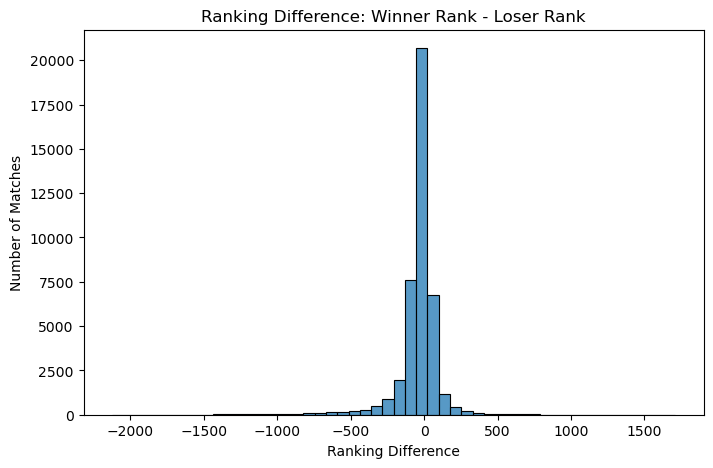
\includegraphics[width=0.82\linewidth]{main_files/main_16_0.png}
  \caption{Distribution of ranking difference, defined as winner rank minus loser rank. Negative values indicate that the winner was better ranked.}
  \label{fig:ranking-diff}
\end{figure}

\subsection{Avoiding target leakage}

The original files are stored from the winner's perspective, with columns such as \texttt{winner\_rank} and \texttt{loser\_rank}. This format is convenient for analysis after the fact, but it is dangerous for prediction because the column names reveal the target. A model should not be given a table where the first player is always the winner. We address this by converting each match to a Player 1 versus Player 2 format and randomly flipping whether the real winner or real loser becomes Player 1. The target variable \texttt{player\_1\_won} is then 1 if Player 1 won and 0 otherwise. The resulting target balance is nearly perfect: 49.9\% Player 1 wins and 50.1\% Player 1 losses.

We also avoid leakage in historical features. For each player, we sort matches by date, tournament identifier, and match number. We then compute cumulative features using only matches before the current match. This means that a player's win rate entering a match does not include the match itself. Same-match serve and return statistics are excluded entirely because they are outcomes of the match rather than pre-match information.

\section{Method}
\label{sec:method}

\subsection{Feature engineering}

The modeling table contains both direct pre-match variables and engineered differences between Player 1 and Player 2. Direct numeric variables include each player's rank, ranking points, age, number of prior matches in the dataset, and the match year. Categorical variables include court surface, round, and best-of format. Difference variables are computed as Player 1 minus Player 2, so a negative rank difference means Player 1 has the better rank, while a positive ranking-points difference means Player 1 has more points.

The most important engineered variables are:
\begin{itemize}
  \item \textbf{Rank difference}: Player 1 rank minus Player 2 rank.
  \item \textbf{Ranking-points difference}: Player 1 ATP ranking points minus Player 2 ranking points.
  \item \textbf{Age difference}: Player 1 age minus Player 2 age.
  \item \textbf{Experience difference}: Player 1 prior match count minus Player 2 prior match count.
  \item \textbf{Career win-rate difference}: difference in each player's pre-match career win rate within the dataset.
  \item \textbf{Recent win-rate difference}: difference in win rate over each player's previous 10 matches.
  \item \textbf{Surface win-rate difference}: difference in each player's pre-match win rate on the same surface.
\end{itemize}

New players with no prior matches are assigned neutral history values of 0.5 for career, recent, and surface win rates. This is a simple smoothing choice: before seeing any evidence in our dataset, we do not assume the player is either stronger or weaker than average. Missing numeric values are imputed with the median inside each model pipeline, and missing categorical values are imputed with the most frequent category before one-hot encoding.

\subsection{Models}

We compare one baseline and three learned models. The baseline predicts that the player with the better ATP rank wins. Because lower numeric ranks are better, the baseline predicts Player 1 wins when \texttt{rank\_diff < 0}. For ROC-AUC, the baseline score is the negative rank difference, so larger scores indicate stronger evidence for Player 1.

The first learned model is logistic regression. It is a useful interpretable baseline because it estimates a linear decision boundary after scaling numeric features and one-hot encoding categorical features. We use class weighting to guard against any small target imbalance, although the randomized Player 1 construction makes the target almost exactly balanced.

The second learned model is a random forest classifier with 250 trees, balanced subsample class weights, and a minimum leaf size of 10. Random forests are well suited to this tabular problem because they can capture nonlinearities without extensive manual feature transformations. The minimum leaf size reduces overfitting to rare players or unusual tournament contexts.

The third learned model is gradient boosting. Boosted trees can be strong on structured tabular data because each new tree focuses on residual errors from the previous ensemble. We include it as a more flexible comparator to logistic regression and random forest, while keeping hyperparameter tuning modest so the comparison remains understandable.

\subsection{Validation design}

We evaluate with \texttt{TimeSeriesSplit} using five splits. Each fold trains on earlier matches and validates on a later slice of the calendar. This is stricter than a random split and better matches the real prediction problem: at prediction time, future results are not available. It also reduces leakage through player history because the model is always tested on matches that occur after the training period.

The main metrics are accuracy, balanced accuracy, F1, precision, recall, and ROC-AUC. Accuracy is the primary metric because the target is balanced and the task is direct winner prediction. Balanced accuracy confirms that a model is not benefiting from class imbalance. F1, precision, and recall show whether the model handles both sides of the randomized Player 1 label well. ROC-AUC evaluates ranking quality independent of one fixed probability threshold.

\section{Evaluation}
\label{sec:evaluation}

\subsection{Baseline behavior}

The ranking-only baseline is strong. Across the five validation folds, it reaches 65.3\% mean accuracy and 0.690 mean ROC-AUC. The fold accuracies range from 63.7\% to 68.0\%. This confirms that rankings capture much of the predictive signal in professional tennis. It also sets a meaningful bar for the learned models: small improvements over this rule still indicate that the engineered features add information, because the baseline is already competitive.

\begin{table}[t]
  \caption{Five-fold time-series cross-validation results. Values are means across folds, with accuracy standard deviation shown to indicate temporal variation.}
  \label{tab:model-results}
  \centering
  \small
  \begin{tabular}{lrrrrrrr}
    \toprule
    Model & Acc. & Acc. SD & Bal. Acc. & F1 & Prec. & Rec. & ROC-AUC \\
    \midrule
    Random Forest & 0.666 & 0.023 & 0.666 & 0.669 & 0.664 & 0.675 & 0.732 \\
    Logistic Regression & 0.660 & 0.022 & 0.660 & 0.662 & 0.658 & 0.666 & 0.724 \\
    Gradient Boosting & 0.656 & 0.012 & 0.656 & 0.659 & 0.654 & 0.666 & 0.721 \\
    Higher-Ranked Baseline & 0.653 & 0.022 & 0.653 & 0.654 & 0.652 & 0.656 & 0.690 \\
    \bottomrule
  \end{tabular}
\end{table}

\subsection{Learned model comparison}

Table~\ref{tab:model-results} summarizes the model comparison. Random forest is the best overall model by mean accuracy and ROC-AUC, reaching 66.6\% accuracy and 0.732 ROC-AUC. Logistic regression is close, at 66.0\% accuracy and 0.724 ROC-AUC. Gradient boosting is slightly lower on accuracy at 65.6\%, though its ROC-AUC of 0.721 still improves over the ranking-only baseline.

The learned models do not crush the baseline, but each of them improves on it in ROC-AUC. This is important because ROC-AUC measures the model's ability to rank likely winners, not just to make a binary call. The random forest's ROC-AUC advantage over the baseline is about 0.042. This suggests that the additional features help the model distinguish between stronger and weaker predictions even when the final accuracy gain is only about 1.4 percentage points.

Figure~\ref{fig:model-comparison} visualizes the same comparison across the metrics. The learned models cluster near one another, while the baseline is especially weaker on ROC-AUC. The pattern supports the interpretation that official rank is an excellent first-order signal, but rank points, historical win rates, and surface information add useful calibration and ordering information.

\begin{figure}[t]
  \centering
  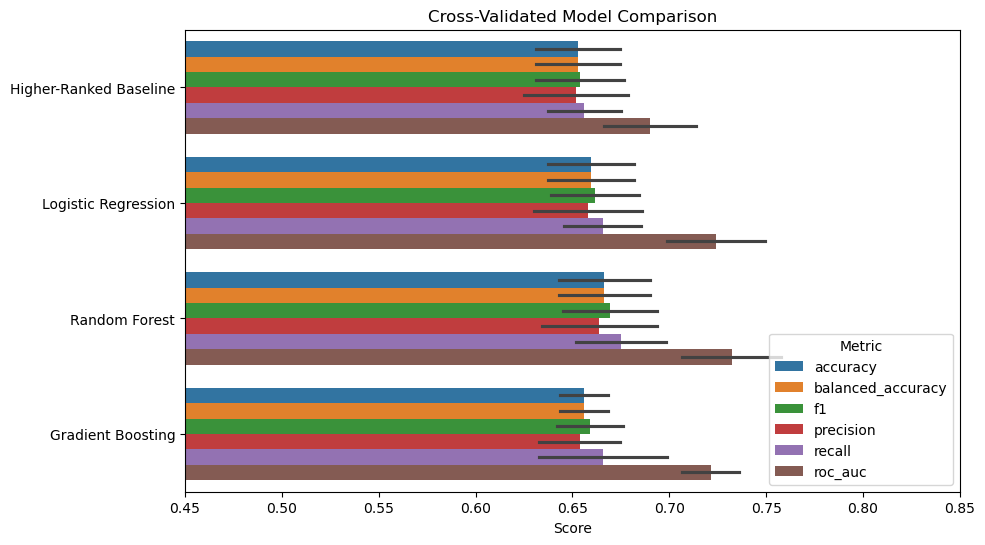
\includegraphics[width=0.95\linewidth]{main_files/main_31_0.png}
  \caption{Cross-validated model comparison across accuracy, balanced accuracy, F1, precision, recall, and ROC-AUC. Bars show mean scores with fold variation.}
  \label{fig:model-comparison}
\end{figure}

\subsection{Feature importance}

To match the example paper's interpretability focus, Table~\ref{tab:feature-importance} reports the strongest random forest features. Ranking-points difference, rank difference, career win-rate difference, and surface win-rate difference are the top four signals. Ranking points preserve more granular information than rank number, while career and surface-specific win rates capture player quality and court specialization that a global rank may miss.

\begin{table}[t]
  \caption{Top random forest feature importances. Difference features are Player 1 minus Player 2.}
  \label{tab:feature-importance}
  \centering
  \small
  \begin{tabular}{rlr}
    \toprule
    Rank & Feature & Importance \\
    \midrule
    1 & Ranking-points difference & 0.126 \\
    2 & Rank difference & 0.105 \\
    3 & Career win-rate difference & 0.098 \\
    4 & Surface win-rate difference & 0.091 \\
    5 & Player 2 ranking points & 0.058 \\
    6 & Experience difference & 0.057 \\
    7 & Player 1 ranking points & 0.057 \\
    8 & Player 1 rank & 0.049 \\
    9 & Player 2 rank & 0.049 \\
    10 & Player 2 prior matches & 0.046 \\
    \bottomrule
  \end{tabular}
\end{table}

Recent form is useful, but it ranks below career and surface history in this model. One explanation is that a 10-match window is noisy, especially when it crosses surfaces or injury recoveries. Categorical surface indicators and round indicators have lower individual importance values, which suggests that surface matters most through player-specific surface history rather than through a generic hard-court or clay-court label alone.

\subsection{Error interpretation}

A 66--67\% accuracy ceiling for these models is plausible. Tennis matches are affected by unobserved conditions that are difficult to infer from public match-level data: injury status, travel fatigue, rest days, matchup style, coaching changes, weather, indoor versus outdoor context, and psychological pressure. Some of these factors may be partially reflected in rankings or recent results, but many are not directly measured in our feature set.

The temporal folds also show performance variation. Both the baseline and learned models are stronger in some folds than others. This may reflect changes in the ATP tour over time, the unusual 2020 season, shifts in the player population, and the fact that some periods contain more established top players while others include more transitions. Time-aware validation makes these shifts visible rather than hiding them inside a random split.

\section{Discussion}
\label{sec:discussion}

The main result is that ranking is hard to beat but not complete. The higher-ranked player wins about two-thirds of the time, and the ranking-only baseline achieves a strong validation accuracy. However, the random forest improves both accuracy and ROC-AUC by combining rank with ranking points, career history, surface history, experience, and age. This supports our original hypothesis that rankings are one of the strongest predictors, while surface and performance-history features provide additional predictive power.

The result also illustrates a common lesson in applied data science: the most complex model is not automatically the best, and the best model is not always dramatically better than a simple baseline. Logistic regression performs only 0.7 accuracy points below random forest, which means much of the signal is close to linear in the engineered difference features. Gradient boosting, despite being flexible, does not outperform random forest in our experiment. With more careful hyperparameter tuning it might improve, but the current comparison is enough to show that model choice matters less than leakage-safe feature construction and realistic validation.

For tennis specifically, ranking points appear more informative than rank alone. This makes sense because rank is ordinal while points are cardinal. The difference between rank 1 and rank 2 may represent hundreds or thousands of points in one season, while the difference between rank 80 and rank 81 may be tiny. Ranking points therefore preserve information about the scale of player separation. The random forest's top feature importance for ranking-points difference is consistent with this reasoning.

Surface-specific win rate is another important finding. Tennis fans often describe players as clay-court specialists, grass-court specialists, or hard-court specialists. Our model finds that a player's prior success on the same surface contributes meaningful predictive signal. This also explains why a global ranking baseline can miss some matches: a lower-ranked player may still be favored in practice if the court surface fits their strengths.

One practical implication is that a simple tennis prediction model should begin with a strong ranking baseline, then add only features that are known before the match and clearly connected to player strength or context. Adding post-match statistics would produce impressive-looking results but would not answer the real prediction question. Our model's modest improvement is more trustworthy precisely because it avoids that shortcut.

\section{Limitations}
\label{sec:limitations}

The project has several limitations. First, the dataset is match-level rather than point-level. It does not include detailed pre-match serve, return, rally, or tactical statistics. We excluded same-match serve and return columns to avoid leakage, but a stronger future model could use rolling pre-match serve and return statistics computed from earlier matches only.

Second, the history features are based only on matches from 2010 onward. Players who were already established at the start of 2010 receive incomplete prior histories, so their early-career features in our table are understated. This affects older players more than newer players. Loading earlier seasons would reduce this cold-start issue.

Third, we do not model head-to-head history, injuries, withdrawals, fatigue, travel, tournament importance, indoor versus outdoor conditions, betting-market expectations, or player handedness. Some of these variables are available in public data, while others would require additional sources or careful manual collection. Their absence likely limits accuracy.

Fourth, our validation is time-aware but still cross-validated on a single historical dataset. It does not provide a true live prospective test on matches after 2024. A stronger evaluation would freeze the model after a chosen date and then evaluate on a later season only once, matching deployment more closely.

Fifth, model tuning is intentionally limited. The random forest and gradient boosting models use reasonable starter settings, not a large hyperparameter search. This keeps the project transparent, but it means the reported numbers should be viewed as a course-project benchmark rather than the best possible ATP prediction system.

Finally, feature importance from random forests should be interpreted cautiously. It indicates which variables the fitted model used, not necessarily causal effects. A feature such as career win-rate difference may be important because it correlates with underlying player quality, not because changing that feature would directly cause a different match outcome.

\section{Conclusion}

We built a leakage-safe ATP match prediction pipeline using public tennis data from 2010 through 2024. The final dataset contains 41,750 cleaned matches rewritten as randomized Player 1 versus Player 2 examples. A higher-ranked-player baseline is already strong, achieving 65.3\% mean time-series cross-validated accuracy. Learned models improve modestly, with random forest performing best at 66.6\% accuracy and 0.732 ROC-AUC. The most informative features are ranking-points difference, rank difference, career win-rate difference, and surface win-rate difference.

The project shows that machine learning can add value beyond official rankings, but it also shows the limits of simple public match-level features. Tennis outcomes are shaped by both stable player strength and short-term conditions that our data only partially observes. A natural next step would be to compute rolling pre-match serve and return statistics, add head-to-head and rest-day features, tune models more systematically, and evaluate on a fully held-out future season.

\clearpage
\begin{thebibliography}{9}
\bibitem[Bradley and Terry(1952)]{bradley1952}
Bradley, R.~A. and Terry, M.~E. (1952).
\newblock Rank analysis of incomplete block designs: I. The method of paired comparisons.
\newblock \emph{Biometrika}, 39(3/4):324--345.

\bibitem[Breiman(2001)]{breiman2001}
Breiman, L. (2001).
\newblock Random forests.
\newblock \emph{Machine Learning}, 45:5--32.

\bibitem[Elo(1978)]{elo1978}
Elo, A.~E. (1978).
\newblock \emph{The Rating of Chessplayers, Past and Present}.
\newblock Arco Publishing.

\bibitem[Friedman(2001)]{friedman2001}
Friedman, J.~H. (2001).
\newblock Greedy function approximation: A gradient boosting machine.
\newblock \emph{The Annals of Statistics}, 29(5):1189--1232.

\bibitem[Pedregosa et~al.(2011)]{sklearn}
Pedregosa, F., Varoquaux, G., Gramfort, A., Michel, V., Thirion, B., Grisel, O., Blondel, M., Prettenhofer, P., Weiss, R., Dubourg, V., Vanderplas, J., Passos, A., Cournapeau, D., Brucher, M., Perrot, M., and Duchesnay, E. (2011).
\newblock Scikit-learn: Machine learning in Python.
\newblock \emph{Journal of Machine Learning Research}, 12:2825--2830.

\bibitem[Sackmann(2026)]{sackmann_atp}
Sackmann, J. (2026).
\newblock ATP tennis rankings, results, and stats.
\newblock \url{https://github.com/JeffSackmann/tennis_atp}. Accessed May 9, 2026.

\end{thebibliography}

\end{document}
